\documentclass[11pt]{article}
\usepackage[margin=.73in]{geometry}
\usepackage{lmodern,amsmath,amssymb,booktabs,graphicx,microtype,fancyhdr,xurl,hyperref,array}
\hypersetup{colorlinks=true,urlcolor=blue,linkcolor=black,pdftitle={HPS GPR v6.4.4: Global probabilities with shifted signal MC}}
\pagestyle{fancy}\fancyhf{}\lhead{HPS GPR: global probabilities with signal MC}\rhead{v6.4.4}\cfoot{\thepage}
\setlength{\headheight}{14pt}\setlength{\parindent}{0pt}\setlength{\parskip}{6pt}\setlength{\emergencystretch}{2em}
\begin{document}
{\LARGE\bfseries Global probabilities\par with the selected signal-MC windows}\par
{\large 2016, 2021 and their combined analysis}\par
25 September 2026\hfill Version 6.4.4

\textbf{The retained raw-statistic baseline.} With the 2016 fit and GP-training exclusion set to $[-2.5,+2.5]u$, its largest observed excess statistic occurs at 91 MeV. The largest statistics for 2021 and for the combined analysis occur at 67 MeV. The original 1,024-scan calibration (cohort A) gives the raw-statistic global probabilities below. Appendices A--D add an independent comparison that calibrates local ranks before searching over mass. Each result uses 1,024 independent simulated experiments, and every experiment is searched over the entire corresponding mass grid.

\begin{center}\small\begin{tabular}{lrrrrr}\toprule
Search & Peak [MeV] & Exceedances & Global $p$ & 95\% MC interval & Global $Z$\\\midrule
2016 & 91 & 67/1024 & 0.066 & [0.051, 0.082] & 1.50\\
2021 & 67 & 239/1024 & 0.234 & [0.208, 0.261] & 0.73\\
Combined & 67 & 202/1024 & 0.198 & [0.173, 0.223] & 0.85\\
\bottomrule\end{tabular}\end{center}

The 2016 local asymptotic value of $3.46\sigma$ becomes $1.50\sigma$ globally; the combined value changes from $2.83\sigma$ to $0.85\sigma$. All three global values are below $2\sigma$ under this calibration.

The quoted $p$ is the add-one estimate $(k+1)/1025$; the interval describes finite-simulation uncertainty in the background exceedance probability. $Z=\max[0,\Phi^{-1}(1-p)]$ expresses the same probability in positive-excess Gaussian units. The probability itself is always reported, including when $Z$ clips to zero.

\textbf{The selected models and mass searches.} Define $u=(m_{\rm rec}-c(m))/s(m)$ using the interpolated MC core center $c$ and width $s$. The MC displacement is already contained in the signal template.

\begin{center}\small\begin{tabular}{lll}\toprule
Search & Signal model and fit/training exclusion & Mass grid [MeV]\\\midrule
2016 & Neighbor MC; $[-2.5,+2.5]u$ & 40--175, step 1\\
2021 & Neighbor MC; $[-4,+3]u$ & 60--240, step 1\\
Combined & Same MC models; retain 2015 Gaussian & 60--240, step 1\\\bottomrule
\end{tabular}\end{center}

The observations are the archived full 2015 and 2016 spectra and the archived 2021 10\% spectrum. The combined fit uses one common signal-strength parameter. All three campaigns contribute through 100 MeV; 2016 and 2021 contribute at 101--175 MeV; only 2021 contributes at 176--240 MeV. Consequently, the combined search is not an all-three-campaign search over its entire domain.

\textbf{The combined physics test.} The combination uses one shared coupling at one generated mass. The individual-year searches are diagnostics; the combination does not choose whichever dataset gives the largest excess. Appendix A verifies the shared-coupling fit. The following appendices compare its raw-statistic and locally calibrated mass searches.

These are conditional global probabilities for the stated grids and a fixed GP background source estimated from the observed spectra. They include the search over mass, but not uncertainty in that source or the earlier choice among windows and signal models. Those limits on interpretation are part of the result.

\clearpage\section*{Raw-statistic baseline: the repeated simulated search}

\textbf{Signal shapes and normalization.} The 2016 template comes from the target-constrained, FEE-smeared and scaled histograms \texttt{h\_MinvScSm\_GeneralLargeBins\_Final\_1}. The 2021 template uses the saved v16 target-constrained MC bank. The saved local Gaussian-plus-affine core fits define the centers and widths; the full empirical histograms define the signal shapes. Between neighboring simulated masses, the core centers and widths are interpolated linearly; the full histogram cumulative probabilities are aligned in $u$ and mixed with the same linear weights. Bin probabilities are differences of this cumulative distribution. At an anchor the original selected MC distribution is recovered. Neither year is extrapolated beyond its adopted MC domain.

Bin centers determine fit membership. The GP is trained on the exterior of the same interval, with no additional excluded region. In 2016, the actual fit bins contain 94.52--97.42\% of the full selected template. The template is not renormalized to this interval: its tails and any probability outside the stored spectrum remain part of its normalization. The 2015 Gaussian and its original $\pm2.25\sigma_{\rm ref}$ interval are retained.

\textbf{The fitted statistic.} The GP uses the training-bin counts to predict the mean background $b$ and covariance in the excluded bins. In count space, write the expected fitted counts as
\[
 \lambda=b+L\eta+\psi S,\qquad \eta\sim N(0,I),\qquad \psi=\epsilon^2/10^{-8}.
\]
Here $LL^\mathsf{T}$ is the regularized GP covariance and $S$ is the binned full-template signal multiplied by the inherited campaign-specific yield conversion. The fit uses Poisson counts and the Gaussian constraint on $\eta$, with positive expected counts. For the combination, campaign background constraints are independent while $\psi$ is common. The free fitted strength is signed. At each mass,
\[
 r(m)=\operatorname{sign}(\widehat\psi)\sqrt{2[\ell(0)-\ell(\widehat\psi)]},
 \qquad q_0(m)=\max[0,r(m)]^2,\qquad T=\max_{m\in\mathcal M}q_0(m),
\]
where $\ell$ is the nuisance-profiled negative log likelihood. The observed peak is selected by this raw statistic, not by a mass-dependent calibrated local probability.

\textbf{The null source.} For each campaign, the archived source is the GP arithmetic-mean spectrum obtained from all observed bins using the saved kernel parameters at a 76 MeV reference mass. It is positive and has been reconstructed numerically from the frozen inputs. It is held fixed when generating independent Poisson counts in every bin. No latent GP function is drawn, and the source is not re-estimated between experiments.

\textbf{The repeated extraction.} A single full-spectrum count draw per campaign and experiment is reused at every mass and in every applicable search. At each mass, the selected exclusion is applied, the GP mean and covariance are recomputed from that draw, and both the free and zero-signal nuisance profiles are fitted. The mass-dependent archived kernel parameters, signal templates and yield conversions remain fixed. This preserves correlations between neighboring mass hypotheses without treating them as independent trials.

For $k$ simulated maxima at least as large as the observed maximum, we report $(k+1)/(N+1)$ alongside $k/N$ in the data tables and an exact two-sided 95\% Clopper--Pearson interval for the exceedance probability. The same simulations also give pointwise local tails. There is no subtraction of a null mean or rescaling of $r$ before constructing the scan maximum.

\clearpage\section*{Raw-statistic baseline: local and global descriptions}
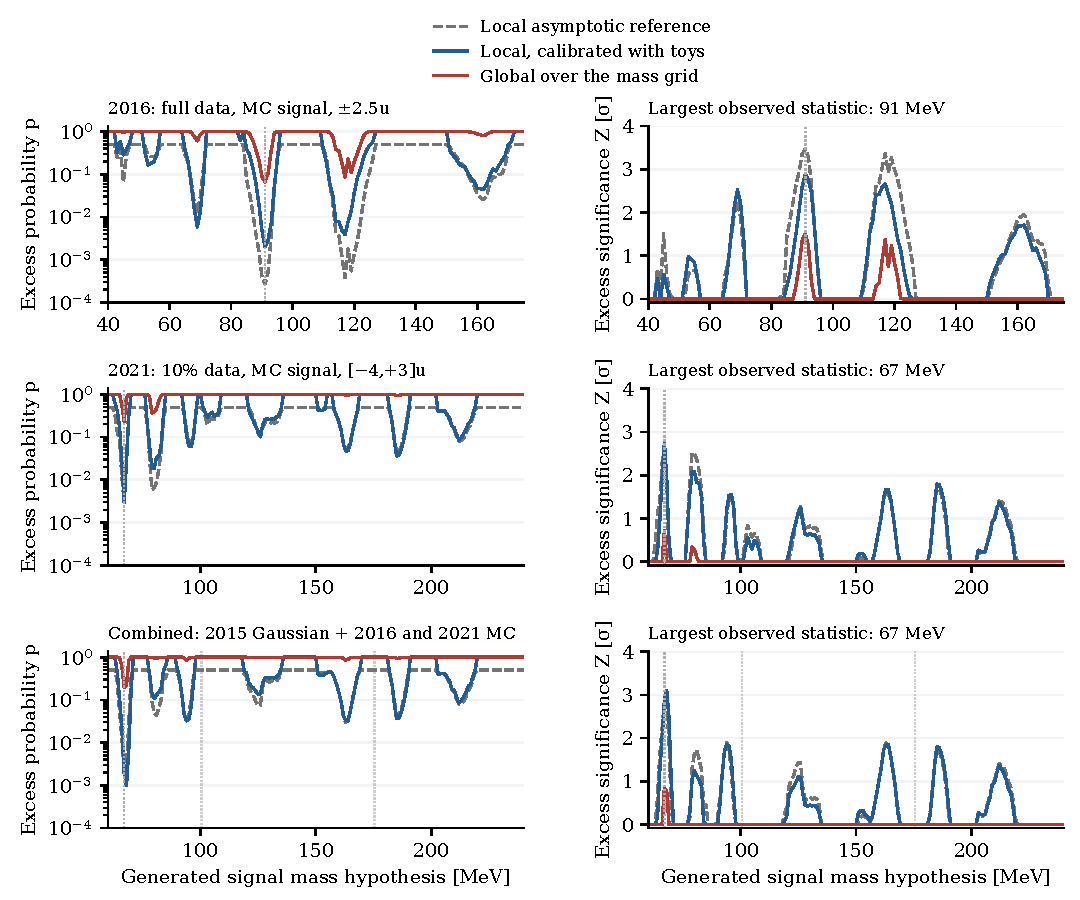
\includegraphics[width=\textwidth]{../figures/local_and_global_scans.pdf}
\refstepcounter{figure}\textbf{Figure \thefigure. How to read the three probability descriptions.} Gray is the inherited fixed-mass asymptotic reference, $p=\Phi[-\max(0,r)]$. Blue compares each observed $q_0(m)$ with simulated $q_0$ at that same mass. Red compares it with the largest simulated $q_0$ anywhere in the corresponding scan. The vertical line marks the largest observed raw statistic; dotted boundaries in the combined row mark changes in the contributing campaigns. All $Z$ values are clipped at zero for $p\ge1/2$; at $q_0=0$, the empirical upper tail includes all ties and equals one.

\begin{center}\small\begin{tabular}{lrrrrr}\toprule
At the selected peak & Asymptotic $Z$ & Local $k/N$ & Local toy $p$ & Local toy $Z$ & Global $Z$\\\midrule
2016 & 3.46 & 1/1024 & 0.0020 & 2.89 & 1.50\\
2021 & 2.74 & 2/1024 & 0.0029 & 2.76 & 0.73\\
Combined & 2.83 & 1/1024 & 0.0020 & 2.89 & 0.85\\
\bottomrule\end{tabular}\end{center}

Blue calibrates each mass; red calibrates the largest raw statistic. Their difference is not a unique look-elsewhere penalty when local null distributions vary with mass: largest raw $q_0$ need not mean smallest local $p$. Appendix B compares both searches. The selected local tails have only one or two exceedances: their 95\% probability intervals are $[0.0000247,0.00543]$ for 2016 and combined, and $[0.000237,0.00704]$ for 2021. Thus small differences between local asymptotic and toy values are not resolved precisely by this sample.

\clearpage\section*{Raw-statistic baseline: the largest background excess}
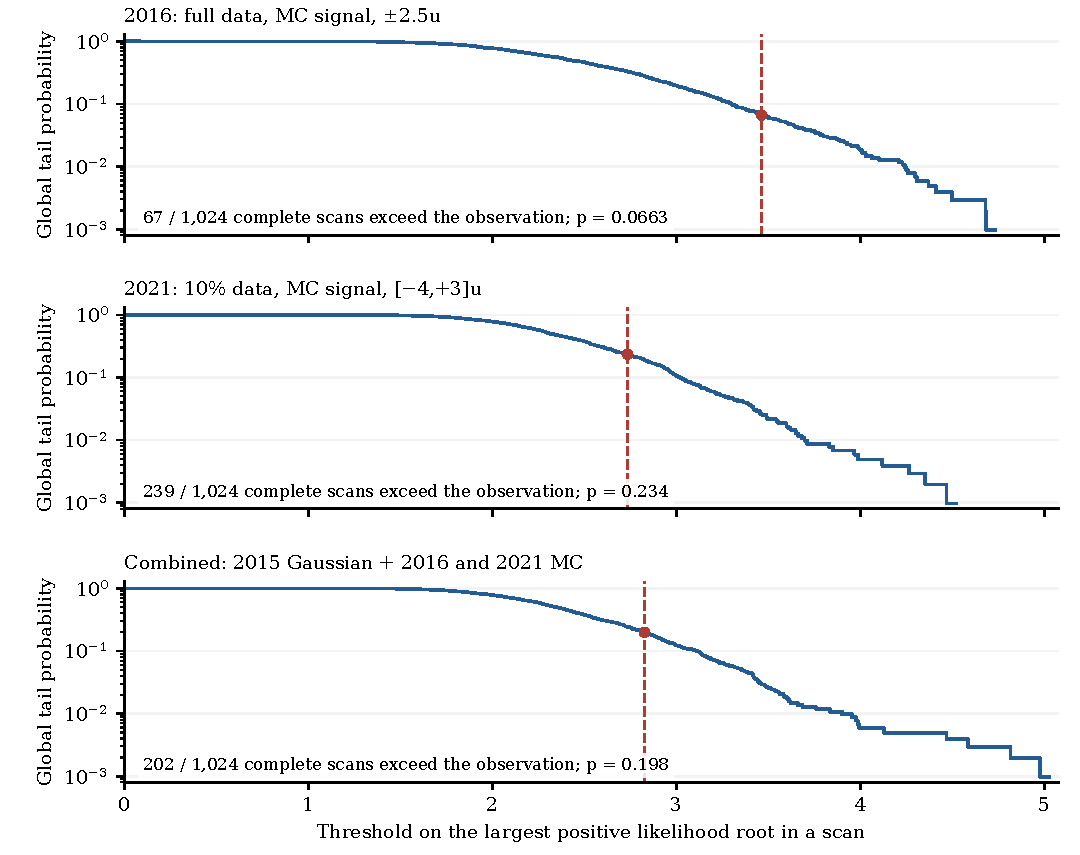
\includegraphics[width=\textwidth]{../figures/scan_maximum_tails.pdf}
\refstepcounter{figure}\textbf{Figure \thefigure. The global probabilities are measured directly.} Blue shows the add-one upper tail of the largest positive likelihood root in each of the 1,024 complete simulated searches. The red line is the observed maximum, and its intersection with the blue curve gives the reported global probability. The finite-simulation floor is $1/1025$; the curve is not extrapolated into an unmeasured tail.

\begin{center}\small\begin{tabular}{lrrr}\toprule
Search & Observed peak [MeV] & Null mean of $r$ at that mass & Null standard deviation\\\midrule
2016 & 91 & +0.648 & 0.957\\
2021 & 67 & +0.093 & 1.027\\
Combined & 67 & -0.031 & 0.968\\
\bottomrule\end{tabular}\end{center}

These pointwise moments help interpret the difference between asymptotic and simulated local probabilities. They are diagnostics of the chosen GP source and extraction, and are not used to recenter the statistic. The global calibration includes their effect automatically. Its finite-simulation interval describes uncertainty from the number of experiments, not uncertainty in the background model or detector response.

\clearpage\section*{Baseline scope, validation and reproducibility}

\textbf{What the baseline probabilities answer.} Under each fixed background source, how often does the extraction produce a largest raw excess statistic at least as large as observed on its 1 MeV grid? The combined row tests one shared coupling. The older across-search calculation remains in \texttt{results/family\_global.json} as an archival diagnostic; it is not the combined physics test. These probabilities do not include the earlier choice among 2016 windows, signal templates or background constructions. The appendix evaluates a second, explicitly defined mass-search statistic.

Because the null source was estimated from the same observed spectra, this study conditions on that estimate. It does not propagate uncertainty in the source or demonstrate that any real signal would be excluded from its construction. The result is also restricted to the finite mass grid; a continuously optimized mass search would require its own calibration. The 2021 input remains the 10\% data sample, without an extrapolation to full luminosity. These calculations therefore do not establish an unconditional physical discovery significance.

\textbf{Relation to the preceding studies.} The neighboring-template construction, archived spectra, kernel settings and common-strength likelihood are inherited from the v6.3.n and v6.4.n studies. The retained baseline selected $\pm2.5u$ for 2016 and recomputed the observed scans and their null calibration. This revision preserves those results and adds 1,024 independent validation scans. The previous $\pm3.5u$ extraction and $\pm2u$ appendix remain preserved. Their upper limits retain those earlier windows; no previous upper-limit curve is relabeled as a $\pm2.5u$ result. This note reports significance rather than a new limit calibration.

\textbf{Validation of the retained baseline.} All 169 frozen input files are verified by SHA-256. The saved arrays contain 1,024 complete experiments at all 136 2016 masses and all 181 masses in each of the 2021 and combined searches, with no failed or discarded fit rows. This corresponds to 443,392 distinct pairs of free and zero-signal profile fits; the combined result above 175 MeV reuses the identical 2021 fit. Maximum score residual was $2.00\times10^{-7}$ and the smallest fitted expected bin count was 120.10. Every expected count was positive.

Validation regenerated every campaign draw from its seed, checked the complete mass arrays against their checkpoints, verified the fit/exclusion masks and full-template normalization, reconstructed all three null sources, and independently replayed 60 saved toy profiles at eight representative masses. All 181 observed 2021 likelihood roots reproduce the preceding MC extraction to within $4.14\times10^{-10}$. The original scan maxima, exceedance counts and confidence intervals were recomputed from the saved arrays; their numerical records remain unchanged. Previously delivered reports were preserved.

\textbf{Files needed to reproduce or inspect the result.} The accompanying source package contains the inputs, protocol hashes, executable scripts, complete toy scan arrays, per-mass checkpoints, figure data and this LaTeX source. \texttt{README.md} gives the bounded two-worker rebuild command. The numerical tables are \texttt{results/global\_summary.csv} and \texttt{results/local\_global\_curves.csv}; \texttt{results/toy\_maxima.csv} records every simulated maximum. \texttt{qa/global\_validation.json} records the numerical checks. The checkpoint signature pins the sample count, random seed, inputs and extraction code, so a resumed run cannot silently mix different analyses.

\textbf{Baseline precision.} Its fixed sample size was chosen before calibration. The add-one tail has resolution $1/1025$; 1,024 experiments cannot establish an extremely small tail probability. Zero exceedances, if encountered, would give a finite upper bound and never zero probability or infinite significance. No additional simulations were selected according to the observed calibration tail.

\clearpage\section*{Appendix A. One shared coupling, then a search over mass}

\textbf{The combination tests one signal hypothesis.} At each common generated mass $m$, campaign $y$ has its own selected template $f_{yi}(m)$ and fixed conversion $K_y(m)$, but every campaign uses the same signal strength $\psi=\epsilon^2/10^{-8}$:
\[
 \lambda_{yi}=b_{yi}+(L_y\eta_y)_i+\psi K_y(m)f_{yi}(m),\qquad
 \mathcal L(\psi,\{\eta_y\};m)=\prod_y\mathcal L_y(\psi,\eta_y;m).
\]
The nuisance vectors are separate. The joint alternative has one common $\psi$ and the joint null fixes that same parameter to zero. Searching over mass changes $m$ for the complete joint fit. It does not select a campaign or add its independently maximized excess statistics. The inherited $ee$-yield normalization and historical display conversion above the dimuon threshold are unchanged; this audit verifies the common parameter, not a new physical normalization.

An independent factorization audit checks the joint profile against the sum of campaign profiles evaluated at the \emph{same} $\psi$. Across 24 profile points at six masses, the largest negative-log-likelihood difference is $6.26\times10^{-13}$. The table illustrates why independent campaign maxima would define a different test.
\begin{center}\small\begin{tabular}{rrrr}\toprule
Mass [MeV] & Joint $\widehat\psi$ & Joint $q_0$ & Sum of individual $q_0$\\\midrule
67 & 643.5 & 7.993 & 11.208\\
68 & 615.1 & 7.722 & 8.005\\
91 & 92.2 & 0.360 & 18.106\\
\bottomrule\end{tabular}\end{center}
At 91 MeV, the individual campaigns prefer different signal strengths, including a negative 2021 fit. The common-strength result is $q_0=0.360$, while adding the individual excess statistics would give 18.106. The latter is not the statistic used anywhere in the combined scan. Campaign support remains the same as on page 1.

\textbf{Calibrate local behavior before ranking masses.} The retained baseline searches for the largest raw $q_0$. The new comparison first uses cohort A, the original 1,024 null scans, to freeze a local upper-tail map at every mass:
\[
 p_{A,m}(q)=\frac{1+\#\{a\in A:q_a(m)\ge q\}}{1025},
 \qquad S=\min_{m\in\mathcal M}p_{A,m}\bigl(q(m)\bigr).
\]
Smaller $S$ is more extreme. The same frozen map is applied to the observations and 1,024 fresh cohort-B scans. Those scans use identical sources and extraction settings, with a disjoint random-number namespace. The global count includes $S_B\le S_{\rm obs}$, including ties; its add-one probability is $(k_B+1)/1025$.

A fixes the maps and the effective-trials approximation described in Appendix C. B neither updates those maps nor tunes that approximation. Each whole campaign draw is reused across masses and applicable searches, preserving their correlations. Both mass-search statistics still use the common-coupling likelihood above; only their ordering of mass hypotheses differs.

\clearpage\section*{Appendix B. Compare the two global calibrations}
\begin{center}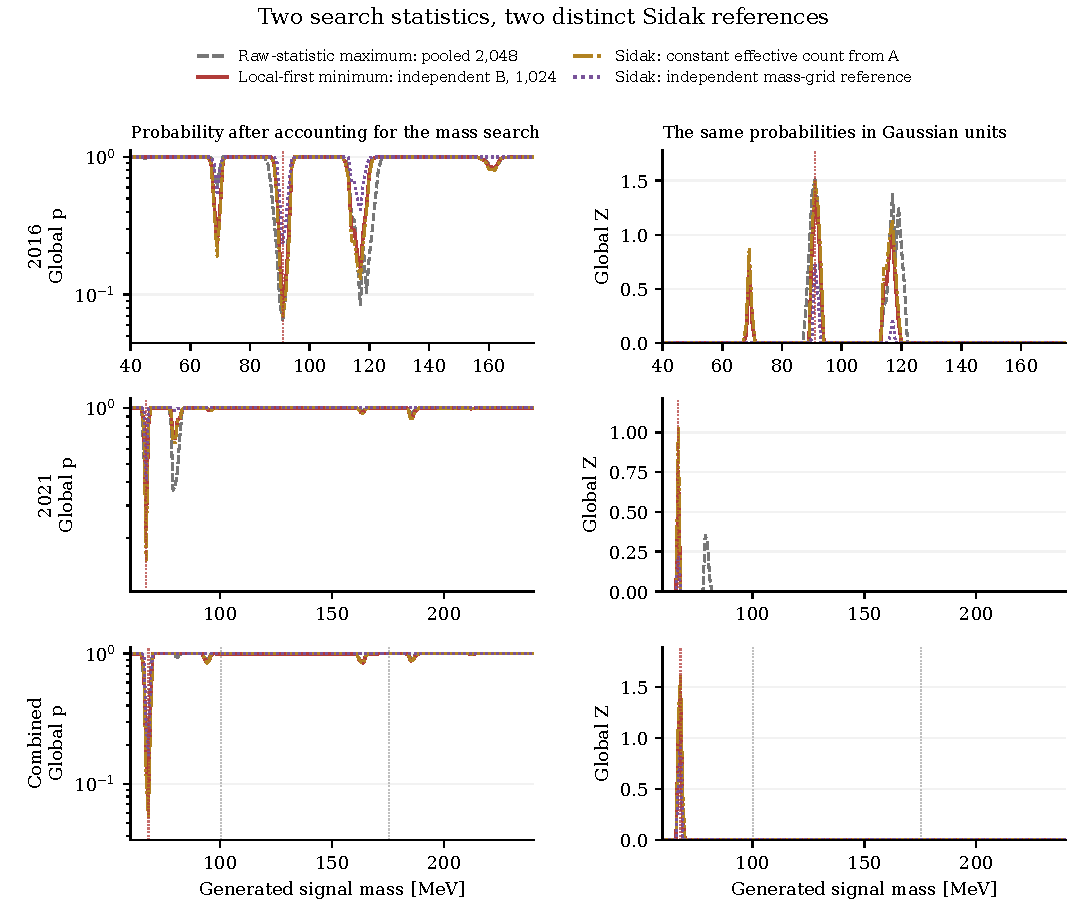
\includegraphics[width=\linewidth,height=4.55in,keepaspectratio]{../figures/calibrated_global_mass_comparison.pdf}\end{center}
{\small\refstepcounter{figure}\textbf{Figure \thefigure. How to read the figure.} Gray compares each observed raw $q_0(m)$ with raw maxima from the pooled 2,048 scans. Red compares its frozen A local rank with the minimum local rank in independent B scans; the red band is a pointwise 95\% interval conditional on A. Gold is the frozen effective-count Sidak approximation. Purple is the independent-mass-grid Sidak reference. The right column expresses the same probabilities as $Z=\max[0,\Phi^{-1}(1-p)]$. Red vertical lines mark the smallest observed local rank; dotted combined boundaries mark campaign changes. Gray and red calibrate different orderings, so neither is a correction factor for the other.}\par\medskip

\begin{center}\small\setlength{\tabcolsep}{4pt}\begin{tabular}{lrrrrrr}\toprule
Search & Peaks: raw/local & Raw pooled $p$ & B count & Local-first $p$ & B 95\% interval & $Z$\\\midrule
2016 & 91 / 91 & 0.065 & 89/1024 & 0.088 & [0.070, 0.106] & 1.35\\
2021 & 67 / 67 & 0.232 & 231/1024 & 0.226 & [0.200, 0.252] & 0.75\\
Combined & 67 / 68 & 0.191 & 75/1024 & 0.074 & [0.058, 0.091] & 1.45\\
\bottomrule\end{tabular}\end{center}

The raw and local-first peaks are each selected using their own declared statistic. For the combined analysis, the raw maximum is at 67 MeV and the smallest calibrated local rank is at 68 MeV. The two procedures ask related but different null-tail questions when the local distributions vary with mass. Their probabilities should be compared as complete procedures rather than choosing whichever reports the smaller value.

All probabilities remain conditional on the fixed GP source and selected extraction. The B interval accounts for its finite number of experiments, holding the A calibration map fixed. It does not include uncertainty in the map, source, signal template or earlier analysis choices. The two Sidak curves are approximations whose independent check appears next.

\clearpage\section*{Appendix C. Two Sidak references with different assumptions}
\begin{center}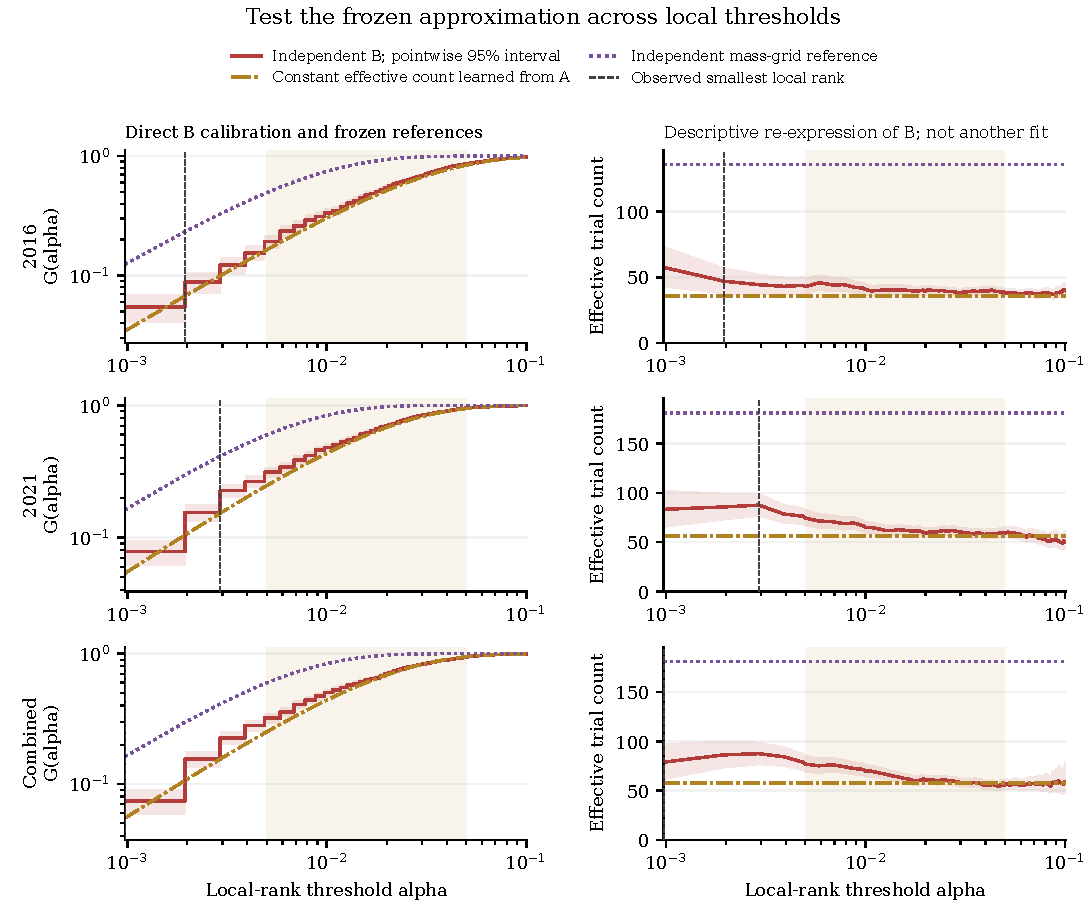
\includegraphics[width=\linewidth,height=4.35in,keepaspectratio]{../figures/calibrated_threshold_comparison.pdf}\end{center}
{\small\refstepcounter{figure}\textbf{Figure \thefigure. How to read the figure.} Left: direct B probabilities $G_B(\alpha)=\Pr(S_B\le\alpha)$ and both Sidak references. Right: $\log[1-G_B(\alpha)]/\log(1-\alpha)$ re-expresses B, with transformed pointwise intervals; it is not another fit. Gold shading marks the A fit range; black lines mark observed local minima. Infinite interval endpoints are omitted. Neither reference resolves probabilities below the A-map floor.}\par\medskip

For independent uniform local probabilities, $G(\alpha)=1-(1-\alpha)^N$. Purple uses the grid size; gold fixes $N_{\rm eff}$ from A alone. A's self-inclusive ranks $\#\{q_A\ge q_i\}/1024$ equal add-one leave-one-out ranks. Their minima are dependent and use different maps from B's full frozen map.

The A-only fit uses equal-weight, zero-intercept least squares of $\log(1-G_A)$ versus $\log(1-\alpha)$ at 0.005, 0.01, 0.02, 0.03 and 0.05. All five thresholds were fixed before B.
\begin{center}\small\begin{tabular}{lrrrrr}\toprule
Search & Grid $N$ & A-fit $N_{\rm eff}$ & Gold $p$ & Purple $p$ & Direct B $p$\\\midrule
2016 & 136 & 35.81 & 0.068 & 0.233 & 0.088\\
2021 & 181 & 56.45 & 0.152 & 0.412 & 0.226\\
Combined & 181 & 57.55 & 0.055 & 0.162 & 0.074\\
\bottomrule\end{tabular}\end{center}
The last three columns use the observed local minima. All gold predictions fall below their direct B 95\% intervals: the constant count understates the global probability here. These are pointwise comparisons, not a simultaneous curve test. These minima are below the fit range, making gold an extrapolation. B's ranks need not be uniform conditional on A; the fitted count describes this estimated-map procedure, not independent windows. The direct B tail is the calibrated global result.

\clearpage\section*{Appendix D. Finite calibration, retained results and references}

\textbf{What the old ``largest selected result'' meant.}\par
That optional diagnostic used $T_{\rm family}=\max(T_{2016},T_{2021},T_{\rm combined})$, where each $T$ already maximizes over mass. It asked whether \emph{any of three displayed searches} looked unusual. It neither defines the joint likelihood nor answers the shared-coupling question. It is archived only. The individual-statistic sum in Appendix A illustrates another different test; neither construction is used for the combined result.

\textbf{The raw-statistic comparison gains an independent cohort.} Because the raw maximum does not depend on a fitted local map, its A and B maxima can be pooled. The table compares the original and fresh cohorts at each raw observed peak. The pooled probability uses 2,048 experiments and denominator 2,049; no B experiment is reused to train a local map.
\begin{center}\small\setlength{\tabcolsep}{4pt}\begin{tabular}{lrrrrrr}\toprule
Search & Mass & A count & A $p$ & B count & B $p$ & Pooled $p$\\\midrule
2016 & 91 & 67/1024 & 0.066 & 66/1024 & 0.065 & 0.065\\
2021 & 67 & 239/1024 & 0.234 & 236/1024 & 0.231 & 0.232\\
Combined & 67 & 202/1024 & 0.198 & 189/1024 & 0.185 & 0.191\\
\bottomrule\end{tabular}\end{center}

\textbf{The local-map floor is part of the result.} A's smallest possible local rank is $1/1025$. The combined observed minimum at 68 MeV attains this floor: no A statistic at that mass reaches the observed one. This does not resolve a zero tail probability or quantify how far beyond A's largest statistic the observation lies. Every B scan reaching the same minimum rank is counted as a tie in the global tail. The direct B result is still defined, but the finite map cannot distinguish more extreme local observations within that last rank category.

The local-first calibration uses only B's 1,024 minima. A's leave-one-out minima are not pooled with them because they use different training maps. Reported intervals are exact two-sided 95\% Clopper--Pearson intervals for the respective exceedance probabilities. At an observed-selected local mass, A's pointwise interval is not a simultaneous confidence statement across the scan. Threshold-derived effective counts in Appendix C are descriptive ratios; they are neither additional significance measurements nor independent confirmation of the fitted constant.

\textbf{Scope and reproducibility.} Both procedures calibrate the specified 1 MeV mass grids under the fixed archived sources. They do not include the earlier selection of the 2016 window, uncertainty in the source estimated from data, or a continuous mass optimization. No new upper-limit calibration is performed. The five-page baseline and its numerical ledgers are retained, including the older across-search diagnostic, but the combined physics result always means one common coupling. The new tables are \texttt{calibrated\_summary.csv}, \texttt{calibrated\_curves.csv}, \texttt{threshold\_comparison.csv} and \texttt{sidak\_fit.json} in \texttt{results/}; protocol records fix the independent cohorts and the A-only fit.

\textbf{Statistical context.} Cowan's discussion explains the distinction between pointwise and search-wide probabilities and the independent-test reference. Gross and Vitells give an asymptotic upcrossing approximation for a search statistic; this appendix uses direct simulated scans and does not implement that approximation. Algeri and collaborators compare look-elsewhere procedures and their finite-sample behavior. These sources motivate separating a defined search calibration from a convenient trial-count approximation:

{\small
G. Cowan, \href{https://www.pp.rhul.ac.uk/~cowan/stat/cowan_lee_25jun21.pdf}{\emph{The Look Elsewhere Effect}}, ODSL Journal Club, 25 June 2021, especially slides 4--12.\par
E. Gross and O. Vitells, \href{https://arxiv.org/abs/1005.1891}{\emph{Trial factors for the look elsewhere effect in high energy physics}}, Eur. Phys. J. C \textbf{70} (2010) 525--530.\par
S. Algeri, D. A. van Dyk, J. Conrad and B. Anderson, \href{https://arxiv.org/abs/1602.03765}{\emph{On methods for correcting for the look-elsewhere effect in searches for new physics}}, JINST \textbf{11} (2016) P12010.\par}
\end{document}
